% !TEX root = ../main.tex
\paragraph{Forward Tagger (FT)}
    The FT extends the capabilities of CLAS12 to detect electrons and photons at the very forward polar angles from $2.5\degree$ to $4.5\degree$.
    The detection of forward-going scattered electrons allows for electroproduction experiments at very low photon virtuality $Q^2$, providing an energy-tagged, linearly polarized, high-intensity, quasi-real photon beam.
    This configuration enables execution of an extensive hadron spectroscopy program.

    \begin{wrapfigure}{l}{0.50\textwidth}
        \centering\frame{
        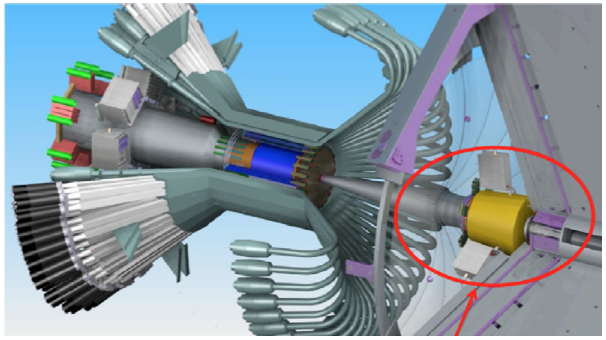
\includegraphics[width=\linewidth]{217ft.png}}
        \caption[FT]{The Forward Tagger system circled downstream of the CD in front of the torus magnet warm bore entrance.}
        \label{fig::ft}
    \end{wrapfigure}

    The FT consists of a calorimeter (FTCal), a micro-strip gas tracker (FTTrk), and a hodoscope (FTHodo).
    The FTCal with 332 lead-tungstate ($\text{PbWO}_4$) crystals is used to identify electrons, measure the electromagnetic shower energy, and provide a fast trigger signal.
    The FTTrk in front of it measures the charged particle scattering angles.
    The scintillator FTHodo aids in separating electrons and high-energy photons.

    During beam operations, a tungsten shielding pipe of conical shape is installed in front of the FT to absorb M\o ller electrons and low-energy photons produced by beam interactions with the target and downstream materials.
    This shield protects both the FT and the Forward Detectors from electromagnetic background.
    The cone angle is $2.5\degree$, such that it is compatible with the FT acceptance.
    In this configuration, known as ``FT-ON'', the FT can be used to detect both electrons and photons, extending the detection capabilities of CLAS12.

    Alternatively, when the FT is not needed for the physics program, the FT detectors are turned off and additional shielding elements are installed in front of the FT covering up to $4.5\degree$ to reduce the background in the DC R1 chambers.
    This configuration, known as ``FT-Off'', reduces the accidental background by one-third at the same beam conditions, which allows for higher luminosity data taking with CLAS12 \cite{acker2020ft}.
    A render of the CD with the FT circled can be seen in Figure \ref{fig::ft}.
